\documentclass[11pt,a4paper]{ltjsarticle}
% Compile with LuaLaTeX

% =========================
% Packages
% =========================
\usepackage{luatexja}
\usepackage{graphicx}
\usepackage{hyperref}
\usepackage{amsmath,amssymb,mathtools}
\usepackage{xcolor}
\usepackage{float}
\usepackage{subcaption}
\usepackage{booktabs}
\usepackage{enumitem}
\usepackage{geometry}

\geometry{margin=22mm}
\setcounter{tocdepth}{3}
\setlength{\parskip}{0.6mm}

% =========================
% User information
% =========================
\title{Weekly Report: Ultra-High-Pressure ODMR --- \\ Does detection-window background flip the green/blue decision?}
\author{Risei Abe}
\date{Week: 2026/07/26 -- 2026/08/01}

% =========================
% Custom commands
% =========================
\newcommand{\sectionblock}[1]{%
  \vspace{2mm}
  {\large\textbf{#1}}
  \vspace{1mm}

}

\newcommand{\todo}[1]{\textcolor{red}{#1}}

\begin{document}

\maketitle

% =========================================================
% 1. Question / Purpose
% =========================================================
\sectionblock{Question}

\begin{quote}
Our lock-in sensitivity model $\eta \propto \Delta\nu/(C\sqrt{R})$ counts only NV photons; does adding the spin-independent background collected in the same $>650$\,nm window (ruby $R$ line, N3/A-band, anvil deformation luminescence) shift the green$\to$blue crossover pressure enough to change which laser we should use at 120\,GPa?
\end{quote}

% =========================================================
% 2. Hypothesis
% =========================================================
\sectionblock{Hypothesis}

If background dilutes contrast and adds shot noise as $\eta = \eta_0\sqrt{1+\rho}$ with $\rho=B/R$, and blue excitation sits in the Cr$^{3+}$ transmission gap (410/555\,nm bands) while shorter blue lines excite N3 more strongly, then the crossover pressure should move with the background-to-signal ratio $\rho_0$ (defined at 532\,nm, ambient) but should not flip green ahead of blue at our 120\,GPa target.

% =========================================================
% 3. Evidence / Interpretation
% =========================================================
\sectionblock{Evidence / Interpretation}

\begin{figure}[H]
  \centering
  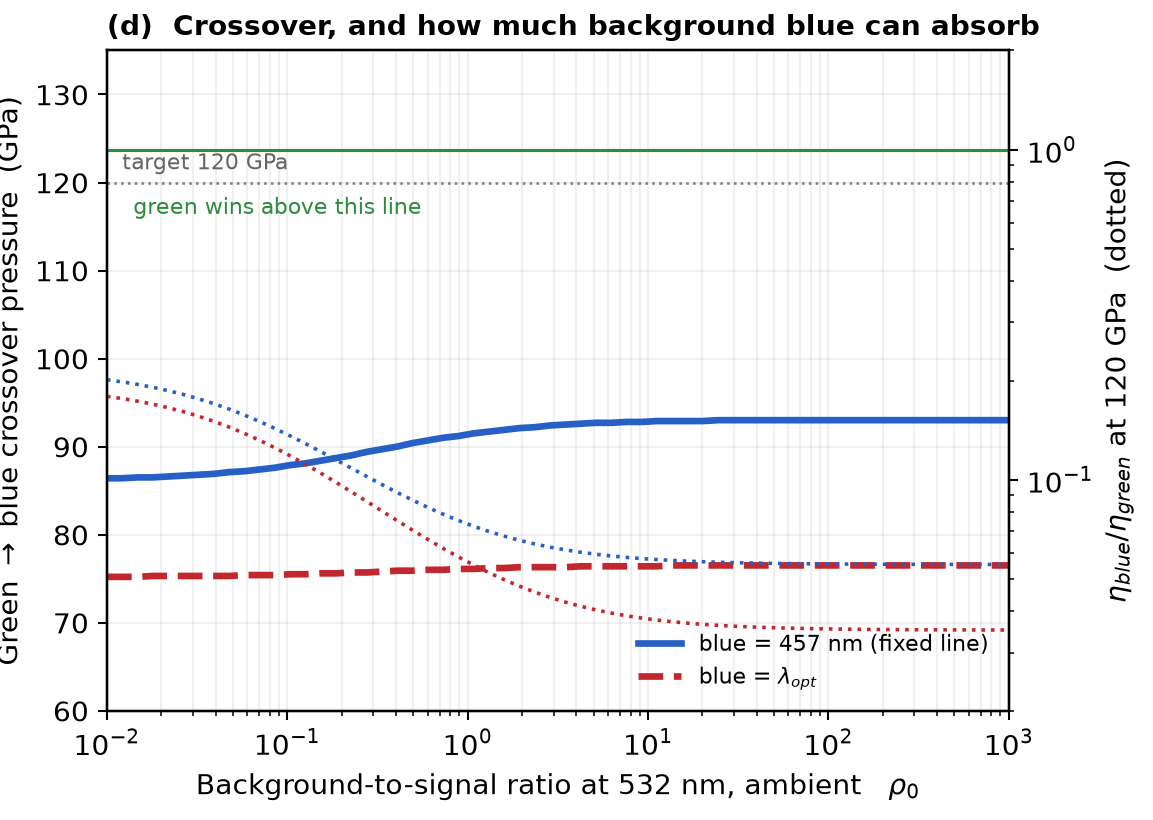
\includegraphics[width=0.46\linewidth]{image/crossover_vs_rho0.png}
  \vspace{-1mm}
  \caption{Green$\to$blue crossover pressure vs.\ background level $\rho_0$, for a fixed 457\,nm blue line and for the pressure-optimal blue wavelength $\lambda_{opt}(\rho_0)$; right axis: $\eta_{blue}/\eta_{green}$ at 120\,GPa.}
  \label{fig:crossover}
\end{figure}
\vspace{-3mm}

\begin{itemize}[leftmargin=8mm]
  \item With 457\,nm fixed, the crossover rises from 86.2\,GPa ($\rho_0{=}0$) to 93.0\,GPa ($\rho_0\to\infty$) because N3 background grows faster toward the near-UV than the Cr$^{3+}$ gap helps at that wavelength.
  \item Using the wavelength-optimized blue line instead, the crossover stays near 75--77\,GPa and $\eta_{blue}/\eta_{green}$ at 120\,GPa falls from 0.194 to 0.035 as $\rho_0\to\infty$, so blue never loses at our operating pressure for any background level.
\end{itemize}

% =========================================================
% 4.  Gap / Failure
% =========================================================
\sectionblock{Gap / Failure}

\begin{itemize}[leftmargin=8mm]
  \item The channel shapes (ruby U/Y bands, N3 edge, broad luminescence) and their mixing weights are phenomenological placeholders, not fit to our anvil, so the crossover numbers are qualitative rather than calibrated.
  \item The absolute background level $\rho_0$ itself is unmeasured, so the model only shows that the conclusion is insensitive to $\rho_0$, not what $\rho_0$ actually is in our cell.
\end{itemize}

% =========================================================
% 5. Next Step
% =========================================================
\sectionblock{Next Step}

Measure the MW-off background spectrum through the $>650$\,nm long-pass under 405/457/532\,nm excitation to pin down $\rho_0$ and the ruby/N3/broad-luminescence split, which also tells us whether ruby-based pressure calibration should be replaced.

% =========================================================
% 9. References
% =========================================================
\sectionblock{References}

\begin{enumerate}[leftmargin=8mm]
  \item K.\,O.\ Ho, C.\ Dailledouze, V.\ \v{Z}alandauskas, \emph{et al.}, ``Optical Stability and Photophysics of NV Centers in Diamond up to 120 GPa,'' arXiv:2606.02399 (2026).
  \item A.\ Dr\'eau \emph{et al.}, Phys.\ Rev.\ B \textbf{84}, 195204 (2011).
  \item Repository: \texttt{code/nv\_bg.py}, \texttt{code/background.py}, \texttt{code/fig5\_background.py} (this analysis).
\end{enumerate}

\end{document}
